\section{Исследовательская часть}

В рамках дипломной работы было проведено исследование сравнения времени обработки и коэффициент сжатия файлов в блочном устройстве zram с оптимизацией и без. Результаты исследования представлены в данном разделе.

\subsection{Описание используемых данных}

Для исследования работоспособности разработанного программного обеспечения и оценки времени обработки данных и коэффициента их сжатия были выбраны бинарные файлы различного типа и разного размера. В исследовании использовались файлы типа pdf (portable document format \cite{pdf}), apk (android package \cite{apk}), случайные файлы из домашней директории, сохраненные в единый файл с помощью утилиты tar \cite{tar}, библиотеки расположенные в корневой директории в папке /lib, так же упакованные с помощью утилиты tar. Сжатие директории /lib с библиотеками является попыткой воспроизвести процесс загрузки библиотек в оперативную память. Размер файлов составляет 400 мегабайт, 430 мегабайт, 5 гигабайт и 17 гигабайт соответственно. Все исследования были проведены для алгоритма сжатия zstd.

\subsection{Вычисление порогового значения энтропии}

Параметр конфигурации ядра CONFIG\_ZRAM\_ENTROPY\_THRESHOLD это некоторое положительное, целое число. Страницы, энтропия которых больше этого параметра, будут помечены как несжимаемые и будут храниться в zram в несжатом виде. Этот параметр задается статически, на стадии сборки ядра, поэтому необходимо подобрать оптимальное значение для каждого из алгоритмов сжатия.

Для определения оптимального порогового значения из модуля ядра zram были собраны данные в формате указанном в таблице 2.

\begin{table}[!htb]
	\label{table:threshold_data}
	\begin{center}
		\caption{Пример csv файла с данными, необходимыми для вычисления параметра CONFIG\_ZRAM\_ENTROPY\_THRESHOLD}
		\begin{tabular}{|c|c|c|c|c|}
			\hline
			\bfseries & \bfseries compressor\_time & \bfseries entropy\_time & \bfseries entropy & \bfseries compress \\ \hline
			0 & 192734 & 6693 & 11502 & 14.2222 \\ \hline
			1 &	565457	& 7364 & 16815 & 6.4341 \\ \hline
			2 & 2591472 & 6975 & 39072 & 3.8496
\\ \hline 
			4 & 1417756 & 5680 & 51755 & 2.4380
\\ \hline
			3 & 1310464 & 5149 & 71668 & 1.8686 \\ 
			\hline
		\end{tabular}
	\end{center}
\end{table}

Каждая строка дает некоторую характеристику странице оперативной памяти, попавшую в блочное устройство zram: 

\begin{itemize}
	\item первый столбец -- номер строки;
	\item второй столбец -- машинное время (в тиках), потраченное на сжатие этой страницы;
	\item третий столбец -- машинное время (в тиках), потраченное на вычисление энтропии для данной страницы;
	\item четвертый столбец -- вычисленное значение энтропии;
	\item пятый столбец -- коэффициент сжатия этой страницы.
\end{itemize}

Все данные в исходном файле отсортированы по коэффициенту сжатия страницы (по возрастанию). На основе этих данных были построены графики формата изображенного на рисунках \ref{fig:compressed_orig} и \ref{fig:compressor_entropy_time}.

\begin{figure}[h]
	\centering
	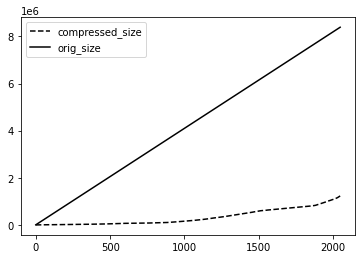
\includegraphics[scale=0.9]{img/compressed_orig.png}
	\caption{Кумулятивные суммы сжатого и несжатого размера страниц}
	\label{fig:compressed_orig}
\end{figure}

На рисунке \ref{fig:compressed_orig} представлены данные о изначальном и сжатом размере страниц. По оси $x$ отложено количество страниц, по оси $y$ размер страниц (в байтах). Прерывистая линия -- кумулятивная сумма столбца compressed\_size (сжатый размер страницы). Сплошная линия -- кумулятивная сумма столбца orig\_size (размер страницы не в сжатом виде).

\begin{figure}[h]
	\centering
	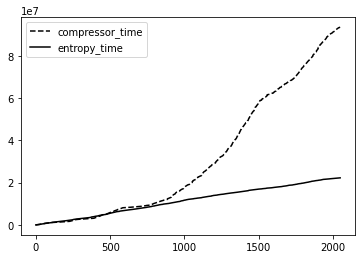
\includegraphics[scale=0.9]{img/compressor_entropy_time.png}
	\caption{Кумулятивные суммы времени затраченного на подсчёт энтропии и сжатия страницы}
	\label{fig:compressor_entropy_time}
\end{figure}

На рисунке \ref{fig:compressor_entropy_time} представлены данные о времени, потраченном на сжатие и вычисление энтропии. По оси $x$ отложено количество страниц, по оси $y$ время (в тиках). Прерывистая линия -- кумулятивная сумма столбца compressed\_size (время, потраченное на сжатие страницы). Сплошная линия -- кумулятивная сумма столбца entropy\_time (время, потраченное на вычисление энтропии).

Проведем прямую из точки графика кумулятивной суммы времени вычисления энтропии, перпендикулярную оси $x$ (см. рис. \ref{fig:compressor_entropy_time}). Примем $x = 1500$ . Проведем второй перпендикуляр к оси $y$ из начала прямой, проведенной как перпендикуляр к оси $x$. На рассматриваемом графике, пересечения второй проведенной прямой и оси $y$ будет в значении $y = 0.7e6$. Далее, необходимо спроецировать верхний график, находящийся справа от первого перпендикуляра до пересечения с точкой начала этой прямой. Пересечение проекции с осью $y$ будет в $y = 4e6$. 

Таким образом, если сжимать лишь страницы, энтропия которых меньше энтропии страницы находящейся в исходных данных под номером 1500 (данные отсортированы по увеличению коэффициенту сжатия), размер сжатых данных будет равен $4e6$ килобайт. В таком случае объем сжатых данных станет больше в два раза, то есть коэффициент сжатия уменьшится в два раза.

Проведем аналогичный перпендикуляр для графика \ref{fig:compressed_orig}, примем $x = 1500$. Можно сделать вывод, что в таком случае, выигрыш по времени составит 25\%. Для данного набора данных можно сделать вывод, что не сжимая страницы, энтропия которых больше энтропии страницы с номером 1500, можно добиться ускорения обработки данных на 25\%, при этом увеличив объем сжатых данных на 200\%.

В результате эксперимента в качестве значения порогового значения энтропии (для алгоритма zstd) было выбрано значение 100 000.

\subsection{Методика проведения исследования}

Для исследования необходимо произвести замеры количества машинных инструкций, времени сжатия и коэффициента сжатия данных с использованием энтропийной оптимизации и без. Количество машинных инструкций и время выполнения подсчитывается с помощью утилиты perf \cite{perf}, а коэффициент сжатия данных с использованием встроенной в модуль zram статистики.

В таблице 3 представлены результаты сравнения коэффициентов сжатия с включенной разработанной оптимизацией и без. В первом столбце указано, включена энтропийная оптимизация или нет. В ячейках таблицы указан исходный размер данных, сжатый и коэффициент сжатия.

\begin{table}[!htb]
	\label{table:coeffs}
	\begin{center}
		\caption{Таблица сравнения коэффициентов сжатия с оптимизаций и без}
		\begin{tabular}{|c|c|c|c|c|}
			\hline
			\bfseries Патч & \bfseries Файл & \bfseries Размер на входе, кб & \bfseries  Размер на выходе, кб & \bfseries Коэф. сжатия \\
			\hline
			Да & pdf & 397.464 & 396.535 & 1.002 \\ 
			Нет & pdf & 397.464 & 395.870 & 1.004 \\ \hline
			Да & apk & 421.340 & 327.992 & 1.284 \\ 
			Нет & apk & 421.340 &  282.331 & 1.492 \\ \hline
			Да & tar & 5.153.692 & 4.131.741 & 1.247 \\ \
			Нет & tar & 5.153.692 & 4.117.655 & 1.251 \\ \hline
			Да & tar (/lib) & 16.527.126 & 5.921.855 & 2.791 \\ \
			Нет & tar (/lib) & 16.527.126 & 5.594.516 & 2.954 \\ \hline
		\end{tabular}
	\end{center}
\end{table}

В таблице 4 представлено сравнение времени выполнения и количества машинных инструкций с включенной оптимизацией и без.

\begin{table}[!htb]
	\label{table:time}
	\begin{center}
		\caption{Таблица сравнения количества машинных инструкций с оптимизаций и без}
		\begin{tabular}{|c|c|c|c|c|}
			\hline
			\bfseries Патч & \bfseries Файл & \bfseries Размер на входе, кб & \bfseries Время сжатия, с& \bfseries Кол-во инструкций \\
			\hline
			Да & pdf & 397.464 & 0.572 & 4.641.658.347 \\ 
			Нет & pdf & 397.464 & 2.098 & 17.187.405.320 \\ \hline
			Да & apk & 421.340 & 1.632 & 13.055.231.312 \\ 
			Нет & apk & 421.340 & 3.196 & 24.345.720.313 \\ \hline
			Да & tar & 5.153.692 & 7.066 & 35.039.839.769 \\ \
			Нет & tar & 5.153.692 & 11.955 & 76.763.123.464 \\ \hline
			Да & tar (/lib) & 16.527.126 & 16.461s & 71.366.805.304 \\
			Нет & tar (/lib) & 16.527.126 & 21.872s & 112.664.002.524 \\ \hline
		\end{tabular}
	\end{center}
\end{table}

\subsection{Вывод}

В результате исследования было установлено что коэффициент сжатия сильно зависит от входных данных. Так, например, файл формата pdf практически не сжался как с включенной энтропийной оптимизацией, так и без.

Было подобран пороговое значения энтропии для алгоритма zstd -- 100 000. Таким образом, страницы, энтропия которых более 100 000 будут храниться в блочном устройстве несжатые. 

Оптимизация метода сжатия ускоряет процесс преобразования данных от 1.5 до 4 раз. Чем меньше процент сжатия исходных данных без включенной оптимизации, тем больше ускоряется процесс сжатия с включенной оптимизацией. Файл формата pdf потерял маленькую долю сжатия (коэффициент сжатия стал 1.002, вместо 1.004), но при этом, процесс преобразования данных ускорился в 4 раза.

Разносортные данные упакованные в единый файл сжимаются в среднем на 25\%. Сжатие с энтропийной оптимизацией происходит в 1.9 раза быстрее, чем без. При этом, потеря в сжатии составляет менее процента.

При сжатии директории /lib, в которой хранятся различные системные библиотеки, 25\%-ый выигрыш по времени достигается с помощью потери 5.5\% сжатого объема (итогового размера).

Подводя итог, можно сделать вывод, что разработанная оптимизация программного обеспечения ускоряет процесс сжатия в несколько раз (1.5-4 раза), при этом потеря в сжатии не крайне малы: от 1\% до 16\%, в зависимости от входных данных. 

Полученные результаты, вместе с модификацией модуля zram, были отправлены в качестве RFC (англ. request for comments \cite{rfc}) письма мейнтейнерам модуля ядра zram \cite{rfc-kernel-patch}.

\pagebreak